\documentclass[12pt]{article}
 \usepackage[margin=1in]{geometry} 
\usepackage{amsmath,amsthm,amssymb,amsfonts}
\usepackage{graphicx} 

\newcommand{\privk}{\text{PrivK}}
\newcommand{\eav}{\text{eav}}
\newcommand{\out}{\text{out}}
\newcommand{\negl}{\text{negl}}
\newcommand{\Enc}{\text{Enc}}
\newcommand{\Dec}{\text{Dec}}
\newcommand{\Gen}{\text{Gen}}
\newcommand{\Mac}{\text{Mac}}
\newcommand{\Vrfy}{\text{Vrfy}}
\newcommand{\Func}{\text{Func}}
\newcommand{\Perm}{\text{Perm}}
\newcommand{\Bingo}{\text{Bingo}}
\newcommand{\Repeat}{\text{Repeat}}
\newcommand{\Newblock}{\text{NewBlock}}
\newcommand{\myn}{l_{in}(n)}

\newcommand{\C}{\mathcal{C}}
\newcommand{\A}{\mathcal{A}}
\newcommand{\OO}{\mathcal{O}}

\newenvironment{problem}[2][Problem]{\begin{trivlist}
\item[\hskip \labelsep {\bfseries #1}\hskip \labelsep {\bfseries #2.}]}{\end{trivlist}}
%If you want to title your bold things something different just make another thing exactly like this but replace "problem" with the name of the thing you want, like theorem or lemma or whatever
 
\begin{document}
%\renewcommand{\qedsymbol}{\filledbox}
%Good resources for looking up how to do stuff:
%Binary operators: http://www.access2science.com/latex/Binary.html
%General help: http://en.wikibooks.org/wiki/LaTeX/Mathematics
%Or just google stuff
 
\title{Chapter 03}
\author{Mingjia Huo}
\date{}
\maketitle

\begin{problem}{3.4}
\begin{proof}
\begin{align*}
    &\Pr[\privk_{\A,\pi}^{\eav}(n)=1]\\
    =&\Pr[b=0]\Pr[\out(\privk_{\A,\Pi}^{\eav}(n,0))=0]+\Pr[b=1]\Pr[\out(\privk_{\A,\Pi}^{\eav}(n,1))=1]\\
    =&\Pr[b=0](1-\Pr[\out(\privk_{\A,\Pi}^{\eav}(n,0))=1])+\Pr[b=1]\Pr[\out(\privk_{\A,\Pi}^{\eav}(n,1))=1]\\
    =&\frac12(\Pr[\out(\privk_{\A,\Pi}^{\eav}(n,1))=1]-\Pr[\out(\privk_{\A,\Pi}^{\eav}(n,0))=1]+1)
\end{align*}
By DEFINITION 3.8, we have
\[ \Pr[\privk_{\A,\Pi}^{\eav}(n)=1]\le\frac12+\negl(n). \]
Additionally, if we have an adversary $\A$ such that $\Pr[\privk_{\A,\Pi}^{\eav}(n)=1]<\frac12-\negl(n)$, by simply inverse the $b'$ $\A$ outputs, we get $\Pr[\privk_{\A,\Pi}^{\eav}(n)=1]>\frac12+\negl(n)$, a contradiction. Thus, DEFINITION 3.8 implies 
$$\Pr[\privk_{\A,\Pi}^{\eav}(n)=1]\ge\frac12-\negl(n).$$
So 
\begin{align*}
    &\text{DEFINITION 3.8}\\
    \Leftrightarrow&\left|\Pr[\privk_{\A,\Pi}^{\eav}(n)=1]-\frac12\right|\le\negl(n)\\
    \Leftrightarrow&\left|\frac12\left(\Pr[\out(\privk_{\A,\Pi}^{\eav}(n,1))=1]-\Pr[\out(\privk_{\A,\Pi}^{\eav}(n,0))=1]+1\right)-\frac12\right|\le\negl(n)\\
    \Leftrightarrow&\left|\Pr[\out(\privk_{\A,\Pi}^{\eav}(n,1))=1]-\Pr[\out(\privk_{\A,\Pi}^{\eav}(n,0))=1]\right|\le\negl(n)\\
    \Leftrightarrow&\text{DEFINITION 3.9},
\end{align*}
which finish the proof.
\end{proof}
\end{problem}

\begin{problem}{3.6}
$ $\par
\textbf{(a). Refute} when $n$ is odd: \par
If $|s|=n=2k+1$ and $l(n)=2n+1$, the length of the output of $G'(s)$ is $l(\lfloor\frac n2\rfloor)=2k+1=|s|$, which contradicts the condition that a pseudorandom generator satisfies $l(n)>n$.\par
\vspace{2ex}
\textbf{Prove} when $n$ is even:\par
By the definition of pseudorandomness, we have: For any PPT algorithm D, there is a negligible function negl such that
\[ \mid\Pr[D(G(s))=1]-\Pr[D(r)=1]\mid\le\negl(n), \]
where $s\in\{0,1\}^n,r\in\{0,1\}^{l(n)}$ are drawn uniformly.\par
So the claim is the same when $s^*\in\{0,1\}^{\lfloor n/2\rfloor},r^*\in\{0,1\}^{l(\lfloor n/2\rfloor)}$.\par
And $G'(s)=G(s_1\cdots s_{\lfloor n/2\rfloor})$, where $s=s_1\cdots s_n$. The length of the output of $G'(s)$ is $l(\lfloor n/2\rfloor)=|r^*|$. So 
\begin{align*}
    &\mid\Pr[D(G'(s))=1]-\Pr[D(r^*)=1]\mid\\
    =&\mid\Pr[D(G(s^*))=1]-\Pr[D(r^*)=1]\mid\\
    \le &\negl(\lfloor n/2\rfloor)\\
    =&\negl(n).
\end{align*}
So $G'(s)$ is a pseudorandom generator.\par\vspace{3ex}
\textbf{(b). Refute}: \par
Using the conclusion in \textbf{(a)}: $G'(s)=G(s_1\cdots s_{\lfloor n/2\rfloor})$ is a pseudorandom generator, where $s=s_1\cdots s_n$. \par
Prove by \textbf{Contradiction}: Assume $G(0^{|s|}\|s)$ is a pseudorandom generator. Then Use the conclusion in \textbf{(a)}, we have $G'(s)=G(0^{|s|})$ also a pseudorandom generator. However, $G(0^{|s|})$ can be easily distinguished from uniform strings. 

Specifically, just let adversary $D$ compare its input with a fixed number $G(0^{n_0})$(Here $n_0$ is a fixed number.) Output $1$ \textit{if and only if} they are equal.

Uniformly choose $s_0\in\{0,1\}^{n_0}$, we have $$\Pr[D(G'(s_0))=1]=\Pr[D(G(0^{|s_0|})=1]=\Pr[D(G(0^{n_0}))=1]=1.$$ 
But randomly select $r_0\in\{0,1\}^{l(n_0)}$, we have $r_0=G(0^{n_0})$ with probability $2^{-l(n_0)}$. So
\[\mid\Pr[D(G'(s_0))=1]-\Pr[D(r_0)=1]\mid=1-2^{-l(n_0)}>\negl(n_0),\]
a contradiction.\par
Thus $G(0^{|s|}\|s)$ is not a pseudorandom generator.\par
\vspace{3ex}
\textbf{(c). Refute}: \par
Prove by \textbf{Contradiction}: 
Assume $G(s)$ is a pseudorandom generator. 
Using the conclusion in \textbf{(a)}, we have $G''(s)=G(s_1\cdots s_{\lfloor n/2\rfloor})$ also a pseudorandom generator. 
However, $G'(s)=G''(s)\|G''(s+1)$ can be easily distinguished from uniform strings. 

Construct $D$: it outputs $1$ \textit{if and only if} the first and second half of the input string is equal.

\begin{itemize}
    \item If the input is $G'(s)$, we have $G'(s)=G''(s)\|G''(s+1)$. However, $G''(s)=G''(s+1)$ when the last $\lceil n/2\rceil$ bits of $s$ is not $11\cdots1$, so the probability is $1-2^{\lceil n/2\rceil}$. That is \[\Pr[D(G''(s))=1]=1-2^{\lceil n/2\rceil}.\]
    \item If the input is $r\in\{0,1\}^{2l(\lfloor n/2\rfloor)}$, we have 
    \[\Pr[D(r)=1]=\Pr[r_0\cdots r_{l(\lfloor n/2\rfloor)}=r_{l(\lfloor n/2\rfloor)+1}\cdots r_{2l(\lfloor n/2\rfloor)}]=2^{\lfloor n/2\rfloor}<\negl(n).\]
    \item So \[\mid\Pr[D(G''(s))=1]-\Pr[D(r)=1]\mid>1-2^{\lceil n/2\rceil}-\negl(n)>\negl(n),\] a contradiction.
\end{itemize}
\end{problem}

\begin{problem}{3.11}
Construct a encryption theme like this:\par
\begin{center}
    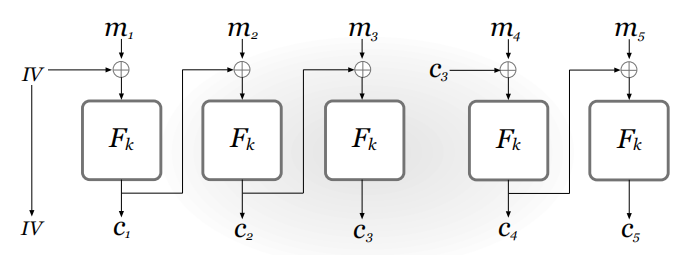
\includegraphics[width=12cm]{1.png}
\end{center}
In this picture, the last block of the previous ciphertext is used
as the $IV$ when encrypting the next message.\par\vspace{2ex}
\textbf{First}, it has indistinguishable multiple encryptions in
the presence of an eavesdropper.\par
Given any adversary $\A$, we can construct a distinguisher $D$ which access an oracle $\OO$:$\{0,1\}^n\rightarrow\{0,1\}^n$. In detail:
\begin{enumerate}
    \item Run $\A(1^n)$. When $\A$ outputs $(m_1^0,\cdots,m_d^0)$ and $(m_1^1,\cdots,m_d^1)$, choose a uniform bit $b\in\{0,1\}$ and then:
    \begin{enumerate}
        \item Get the last ciphertext $c_0$ in the previous encryption(If this is the first encryption, randomly choose $c_0=IV\in\{0,1\}^n$ with uniform distribution.)
        \item Query $\OO(c_0\oplus m_1)$ and obtain response $c_1$, then Query $\OO(c_1\oplus m_2)$ and obtain response $c_2$,\par
        $\cdots$ \par
        until it gets $(c_1,\cdots,c_d)$.
        \item Return $(c_0,c_1,\cdots,c_d)$ to $\A$.
    \end{enumerate}
    \item  A outputs a bit $b'$. Output $1$ if $b'=b$, and $0$ otherwise. 
\end{enumerate}
Thus, $D$ outputs $1$ \textit{if and only if} $\A$ succeeds. Let $\Pi$ denotes our construction, and $\widetilde{\Pi}$ denotes the theme when we replace $F_k$ with a truly random function $f$. Then:
\[\Pr[\privk_{\A,\Pi}^{mult}(n)=1]=\Pr_{k\leftarrow\{0,1\}^n}[D^{F_k(\cdot)}(1^n)=1],\]
\[\Pr[\privk_{\A,\widetilde{\Pi}}^{mult}(n)=1]=\Pr_{f\leftarrow\Func_n}[D^{f(\cdot)}(1^n)=1].\]
By the definition of pseudorandom function, we have 
\[\mid\Pr[D^{F_k(\cdot)}(1^n)=1]-\Pr[D^{f(\cdot)}(1^n)=1]\mid\le\negl(n).\]
Thus
\[\mid\Pr[\privk_{\A,\Pi}^{mult}(n)=1]-\Pr[\privk_{\A,\widetilde{\Pi}}^{mult}(n)=1]\mid\le\negl(n).\]
To prove $\Pr[\privk_{\A,\Pi}^{mult}(n)=1]\le\frac12+\negl(n),$ we only need to prove:\[\Pr[\privk_{\A,\widetilde{\Pi}}^{mult}(n)=1]\le\frac12+\negl(n)\]
We should know that $\Enc_{c_0}(m_1,\cdots,m_d)=f(m_1\oplus c_0, m_2\oplus c_1,\cdots,m_d\oplus c_{d-1})=f(m_1',\cdots,m_d')=(c_1,\cdots,c_d)$. Since $f$ is a random function, given $c\in\{0,1\}^n$, the probability of $f(\cdot)=c$ is $2^{-n}$. ($f$ is uniformly drawn from the set of all functions of $\{0,1\}^n\rightarrow\{0,1\}^n$.)

Define event $\Repeat$ which denotes that there exits $i\ne j\in\{1,2\cdots,n\}$ such that $c_{i}\oplus m_{i+1}=c_j\oplus m_{j+1}$. If there is no $\Repeat$, then answer $(c_1,\cdots,c_d)$ is just a stream of uniform bits. So
\begin{align*}
    &\Pr[\privk_{\A,\widetilde{\Pi}}^{mult}(n)=1]\\
    =&\Pr[\privk_{\A,\widetilde{\Pi}}^{mult}(n)=1\land\Repeat]+\Pr[\privk_{\A,\widetilde{\Pi}}^{mult}(n)=1\land\overline{\Repeat}]\\
    \le&\frac{\OO(d)}{2^n}+\frac12\\
    =&\frac12+\negl(n).\text{\ \ \ \ \ ($d$ is polynomial of n.)}
\end{align*}
Thus,
\[\Pr[\privk_{\A,\Pi}^{mult}(n)=1]\le\frac12+\negl(n).\]
which means the theme has indistinguishable multiple encryptions in
the presence of an eavesdropper.\par
\par\vspace{2ex}
\textbf{Second}, it's not CPA-secure.\par
Construct an adversary $\A$: 
\begin{enumerate}
    \item $\A$ randomly select two different string $m_0,m_1\in\{0,1\}^n$ and output them.
    \item A uniform bit $b\in\{0,1\}$ is chosen, then a ciphertext $c=\Enc_k(m_b)=(IV,c)$ is computed and given to $\A$.
    \item $\A$ compute $m_2=m_0\oplus IV\oplus c$, and get access to $c_2=\Enc_k(m_2)$.
    \item If $c=c_2$, $\A$ outputs $0$; otherwise outputs $1$.
\end{enumerate}
When $b=0$, then $m_0\oplus IV=m_2\oplus c$. Thus the input of $F_k$ is the same, and $c=c_2$ with probability $1$. When $b=1$, $c\ne c_2$ with high probability($1-2^{-|c|}$). So $\A$ succeeds with probability near $1$, which indicates that this theme is not CPA-secure.\par
\end{problem}

\begin{problem}{3.18}
How to decrypt: Given $k\in\{0,1\}^n,c$, compute $m'=F_k^{-1}(c)$. Message $m$ is the second half of $m'$.\par
\textbf{PART 1}: CPA-secure\par
\begin{proof}
Without loss of generality, assume the permutation is fixed length 
Given any adversary $\A$, we can construct a distinguisher $D$ which access an oracle $\OO$:$\{0,1\}^{n}\rightarrow\{0,1\}^{n}$. In detail:
\begin{enumerate}
    \item Run $\A(1^{2n})$. When $\A$ queries its encryption oracle on a message $m\in \{0,1\}^{n}$, answer this query in the following way:
    \begin{enumerate}
        \item choose uniform $r\in\{0,1\}^n$.
        \item Query $\OO(r\|m)$ and obtain response $y$.
        \item Return the ciphertext $y$ to $\A$.
    \end{enumerate}
    \item When $\A$ outputs messages $m_0,m_1\in\{0,1\}^n$, choose a uniform bit $b\in\{0,1\}$ and then:
    \begin{enumerate}
        \item choose uniform $r_0\in\{0,1\}^n$.
        \item Query $\OO(r_0\|m_b)$ and obtain response $y$.
        \item Return the ciphertext $y$ to $\A$.
    \end{enumerate}
    \item Continue answering encryption-oracle queries of $\A$ as before
until $\A$ outputs a bit $b'$. Output $1$ if $b'=b$, and $0$ outherwise.
\end{enumerate}

Thus, $D$ outputs $1$ \textit{if and only if} $\A$ succeeds. Let $\Pi$ denotes our construction, and $\widetilde{\Pi}$ denotes the theme when we replace $F_k$ with a uniform permutation $f\in\Perm_n$. Then:
\[\Pr[\privk_{\A,\Pi}^{cpa}(2n)=1]=\Pr_{k\leftarrow\{0,1\}^{2n}}[D^{F_k(\cdot)}(1^{2n})=1],\]
\[\Pr[\privk_{\A,\widetilde{\Pi}}^{cpa}(2n)=1]=\Pr_{f\leftarrow\Perm_{2n}}[D^{f(\cdot)}(1^{2n})=1].\]
By the definition of pseudorandom permutation, we have 
\[\mid\Pr[D^{F_k(\cdot)}(1^{2n})=1]-\Pr[D^{f(\cdot)}(1^{2n})=1]\mid\le\negl(2n).\]
Thus
\[\mid\Pr[\privk_{\A,\Pi}^{cpa}(2n)=1]-\Pr[\privk_{\A,\widetilde{\Pi}}^{cpa}(2n)=1]\mid\le\negl(2n),\]
that is 
\[\mid\Pr[\privk_{\A,\Pi}^{cpa}(n)=1]-\Pr[\privk_{\A,\widetilde{\Pi}}^{cpa}(n)=1]\mid\le\negl(n).\]
To prove $\Pr[\privk_{\A,\Pi}^{cpa}(n)=1]\le\frac12+\negl(n),$ we only need to prove:\[\Pr[\privk_{\A,\widetilde{\Pi}}^{cpa}(n)=1]\le\frac12+\negl(n)\]\par
Define event $\Repeat$ which denotes $r_0$ was selected in some query. (There are totally $d=q(n)$ queries.) If there is no $\Repeat$, then answer $c$ is just uniform bits. So
\begin{align*}
    &\Pr[\privk_{\A,\widetilde{\Pi}}^{cpa}(n)=1]\\
    =&\Pr[\privk_{\A,\widetilde{\Pi}}^{cpa}(n)=1\land\Repeat]+\Pr[\privk_{\A,\widetilde{\Pi}}^{cpa}(n)=1\land\overline{\Repeat}]
\end{align*}
Separately,
\begin{enumerate}
    \item $\Pr[\privk_{\A,\widetilde{\Pi}}^{cpa}(n)=1\land\Repeat]$: \par
    Since $r$ is drawn uniformly, the above probability is $\frac{\OO(d)}{2^{n}}=\negl(n)$.\par
    \item Let $R_{asked}$ denote the set of $r$ used by the experiment during the queries. And $R$ denotes the event that which $r$ is chosen.
    \begin{align*}
        &\Pr[\privk_{\A,\widetilde{\Pi}}^{cpa}(n)=1\land\overline{\Repeat}]\\
        =&\Pr[\privk_{\A,\widetilde{\Pi}}^{cpa}(n)=1\mid\overline{\Repeat}]\times \Pr[\overline{\Repeat}]\\
        =&\Pr[\overline{\Repeat}]\sum_{r\not\in R_{asked}}\Pr[R=r](\Pr[\Enc(r\|m_0)=c]\Pr[b=0]+\Pr[\Enc(r\|m_1)=c]\Pr[b=1])\\
        =& \Pr[\overline{\Repeat}]\sum_{r\not\in R_{asked}}\Pr[R=r](\Pr[\Enc(r\|m_1)=c]\Pr[b=0]+\Pr[\Enc(r\|m_0)=c]\Pr[b=1])\\
        =&\Pr[\privk_{\A,\widetilde{\Pi}}^{cpa}(n)=0\land\overline{\Repeat}]
    \end{align*}
    So \[\Pr[\privk_{\A,\widetilde{\Pi}}^{cpa}(n)=1\land\overline{\Repeat}]=\frac12\]
\end{enumerate}
Thus,
\begin{align*}
    &\Pr[\privk_{\A,\widetilde{\Pi}}^{cpa}(n)=1]\\
    =&\Pr[\privk_{\A,\widetilde{\Pi}}^{cpa}(n)=1\land\Repeat]+\Pr[\privk_{\A,\widetilde{\Pi}}^{cpa}(n)=1\land\overline{\Repeat}]\\
    \le&\frac12+\negl(n)
\end{align*}
which means CPA-secure.\par
\end{proof}
\textbf{PART 2}: The proof of CCA-secure is the same with problem $4.25$.
\end{problem}

\begin{problem}{3.29}
Define when given $1^n$ to Gen, the message is $l_{in}(n)$ in length, which is polynomial in $n$. For that reason, we can assume $l_{in}(n)=n$, which don't affect the result of $\negl(n)$.  
Construct a theme $\Pi=(\Gen, \Enc, \Dec)$ as followed:
\begin{enumerate}
    \item Gen: on input $1^n$, choose $(k_1,k_2)$ based on the $\Gen_1(1^n), \Gen_2(1^n)$ in $\Pi_1, \Pi_2$. 
    \item Enc: Given $m\in\{0,1\}^n$, uniformly select a $m_l\in\{0,1\}^n$. Then compute $m_r=m\oplus m_l$. Use $\Enc_1^{k_1}$ to encrypt $m_l$ and $\Enc_2^{k_2}$ to encrypt $m_r$. The ciphertext we get is $(c_1,c_2)$.
    \item Dec: $m=\Dec_1^{k_1}(c_1)\oplus \Dec_2^{k_2}(c_2).$
\end{enumerate}
\begin{proof}
Now we prove it's CPA-secure.\par
Assume there is an adversary $\A$ for $\Pi$. Construct an adversary $\A_2$ for $\Pi$ as followed:
\begin{enumerate}
    \item $\A_2$ has oracle $\Enc_{k_2}(\cdot)$, with $k_2$ unknown to $\A_2$. But $\A_2$ can choose $k_1\leftarrow\Gen_1(1^n)$, then construct a new oracle $$\Enc_{k_1,k_2}(\cdot)=(\Enc_{k_1}(m_l),\Enc_{k_2}( m_l\oplus\cdot)).$$ Here $m_l\in\{0,1\}^n$ is uniformly selected by the oracle.
    \item $\A$ queries the oracle $\Enc_{k_1,k_2}(\cdot)$ and get the ciphertexts. 
    \item $\A$ asks $m_0',m_1'$. Then $\A_2$ uniformly choose $m_l\in\{0,1\}^n$, construct $(m_0,m_1)=(m_l\oplus m_0',m_l\oplus m_1')$ and ask the CPA-experiment. Then $\A_2$ get $c$, and pass $(\Enc_{k_1}(m_l),c)$ to $\A$. 
    \item $\A$ asks some queries to $\Enc_{k_1,k_2}(\cdot)$ and output $b'\in\{0,1\}$.
    \item $\A_2$ output $b'$. 
\end{enumerate}
In this experiment, both $\A$ and $\A_2$ don't know $b$, and what $\A_2$ guesses is the same as what $\A$ guesses. Also, 
\begin{align*}
    &\privk_{\A_2,\Pi}^{cpa}(n)=1\\
    \Leftrightarrow &c=\Enc_{k_2}(m_{b'})\\
    \Leftrightarrow &(\Enc_{k_1}(m_l),c)=(\Enc_{k_1}(m_l),\Enc_{k_2}(m_l\oplus m_{b'}'))\\
    \Leftrightarrow&\privk_{\A,\Pi}^{cpa}(n)=1.
\end{align*}
So \[\Pr[\privk_{\A_2,\Pi}^{cpa}(n)=1]=\Pr[\privk_{\A,\Pi}^{cpa}(n)=1].\]
Similarly, we can construct an adversary $\A_1$ such that 
\[\Pr[\privk_{\A_1,\Pi}^{cpa}(n)=1]=\Pr[\privk_{\A,\Pi}^{cpa}(n)=1].\]
So if $\Pi$ is not CPA-secure, then 
$\exists\A,s.t.\Pr[\privk_{\A,\Pi}^{cpa}(n)=1]>\frac12+\negl(n)$, so \[\Pr[\privk_{\A_2,\Pi}^{cpa}(n)=1]=\Pr[\privk_{\A_1,\Pi}^{cpa}(n)=1]>\frac12+\negl(n),\]
which means that each of $\Pi_1$ and $\Pi_2$ is not CPA-secure, a contradiction.\par
Thus $\Pi$ is CPA-secure.
\end{proof}
\end{problem}

\end{document}